% 2007 年新课标卷文科第 22 题：圆的切线 AP、割线 ABC、弦 BC 中点 M。
%   圆 O 半径 2，A(-4,0)，切点 P=(-1,√3)；
%   割线 ABC 从 A 出发，B、C 为与圆的交点，M 为 BC 中点。
% 来源 PDF：gaokaomath-src/普通高考/2007/2007新课标文(海南,宁夏).pdf
% SHA-256：c8ee1632ac3a7a28aab1150f047a2e1c74398ca2944701e9165237897ae724e2
% 原页：2007新课标文(海南,宁夏).pdf 第 2 页（A3 三栏）第 3 栏，书页码 394。
% 重绘依据：按原页点、线与圆的位置重绘；A-O 与 P-M 为题目用到的辅助线。
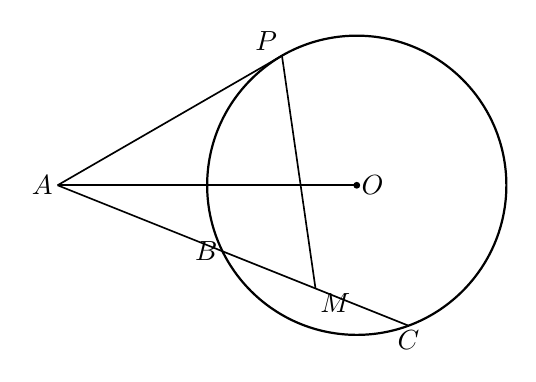
\begin{tikzpicture}[scale=0.95, semithick,
  every node/.style={inner sep=1.5pt}]

  \coordinate (O) at (0,0);
  \coordinate (A) at (-4,0);
  \coordinate (P) at (-1,1.732);
  \coordinate (B) at (-1.795,-0.882);
  \coordinate (C) at (0.692,-1.877);
  \coordinate (M) at (-0.5515,-1.3795);

  \draw[thick] (O) circle (2);
  \fill (O) circle (1.3pt);

  % 切线、割线与辅助线
  \draw (A) -- (P);
  \draw (A) -- (C);
  \draw (A) -- (O);
  \draw (P) -- (M);

  \node[left] at (A) {$A$};
  \node[above left] at (P) {$P$};
  \node[right] at (O) {$O$};
  \node[left] at (B) {$B$};
  \node[below] at (C) {$C$};
  \node[below right] at (M) {$M$};
\end{tikzpicture}
